\documentclass[logo,reportComp]{thesis}
\usepackage[cpp,pseudo]{mypackage}

\title{操作系统原理实验报告}
\subtitle{实验四:中断处理与系统调用}
\school{数据科学与计算机学院}
\author{陈鸿峥}
\classname{17大数据与人工智能}
\stunum{17341015}
\headercontext{操作系统原理实验报告}
% \authorremark{本实验报告用\LaTeX撰写,创建时间:\builddate\today}

\begin{document}

\maketitle

\section{实验目的}
\begin{itemize}
	\item 学习中断中断机制知识,掌握中断处理程序设计的要求
	\item 学习通过汇编程序实现时钟中断处理
\end{itemize}

\section{实验要求}
% 实验目的和实验要求由老师提供实验项目文档中获取
\begin{itemize}
	\item % 操作系统工作期间,利用时钟中断,在屏幕最边缘处动态画框,第一次用字母A,第二次画用字母B,如此类推,还可加上变色闪耀等效果。适当控制显示速度,以方便观察效果。
	操作系统工作期间,利用时钟中断,在屏幕24行79列位置轮流显示`|'、`/'和`\verb'\'',适当控制显示速度,以方便观察效果。
	\item 编写键盘中断响应程序,原有的你设计的用户程序运行时,键盘事件会做出有事反应:当键盘有按键时,屏幕适当位置显示``OUCH! OUCH!''。
	\item 在内核中,对33号、34号、35号和36号中断编写中断服务程序,分别在屏幕1/4区域内显示一些个性化信息。
	再编写一个汇编语言的程序,作为用户程序,利用\verb'int 33'、\verb'int 34'、\verb'int 35'和\verb'int 36'产生中断调用你这4个服务程序。
	% \item 扩充系统调用,实现三项以上新的功能,并编写一个测试所有系统调用功能的用户程序。
\end{itemize}

\section{实验环境}
% 包括:硬件或虚拟机配置方法、软件工具与作用、方案的思想、相关原理、程序流程、算法和数据结构、程序关键模块,结合代码与程序中的位置位置进行解释。不得抄袭,否则按作弊处理。
% 实验方案包括相关基础原理、实验工具和环境、程序流程和算法思想、数据结构与程序模块功能说明,代码文档组成说明等
具体环境选择原因已在实验一报告中说明。
\begin{itemize}
	\item Windows 10系统 + Ubuntu 18.04(LTS)子系统
	\item gcc 7.3.0 + nasm 2.13.02 + GNU ld (Binutils) 2.3.0
    \item GNU Make 4.1
	\item Oracle VM VirtualBox 5.2.8
    \item Bochs 2.6.9
	\item Sublime Text 3
\end{itemize}

虚拟机配置:内存4M,无硬盘,1.44M虚拟软盘引导。

\section{实验方案}
% 包括:主要工具安装使用过程及截图结果、程序过程中的操作步骤、测试数据、输入及输出说明、遇到的问题及解决情况、关键功能或操作的截图结果。不得抄袭,否则按作弊处理。
本次实验的关键在于写中断向量表。
中断向量表存放在物理地址\verb'0x0000'到\verb'0x03ff',大小为1KB(1024B)。
每个中断在中断向量表中占輴轂,高位为中断处理程序的段地址,低位为中断处理程序的偏移量。
且每个中断对应着一个中断标号,计算标号为$i$的中断入口地址可以通过$4\times i$得到。

而写向量表的操作,我已在实验二中实现宏汇编代码,因此本次实验复用就比较简单。

\subsection{时钟中断}
需要通过可编程中断控制器(Programmable Interrupt Controller, PIC)(见下表),实现中断响应。
\begin{center}
\begin{tabular}{cccc}\hline
PIC 1 & 硬件中断 & PIC 2 & 硬件中断\\\hline
0 & 时钟 & 8 & 实时钟\\
1 & 键盘 & 9 & 通用IO\\
2 & PIC 2 & 10 & 通用IO\\
3 & COM 2 & 11 & 通用IO\\
4 & COM 1 & 12 & 通用IO\\
5 & LPT 2 & 13 & 协处理器\\
6 & 软盘 & 14 & IDE总线\\
7 & LPT 1 & 15 & IDE总线\\\hline
\end{tabular}
\end{center}

具体到时钟中断,即对8号中断进行編程。
将\verb'0x08'放入\verb'0x20'的位置,处理时钟中断函数的入口放入\verb'0x22'。
注意时钟中断最后要告诉硬件端口已经处理完中断,并正常返回,见下面程序。
\begin{lstlisting}[language={[x86masm]Assembler}]
push eax
mov al, 20h
out 20h, al
out 0A0h, al
pop eax
iret
\end{lstlisting}

实现无敌风火轮则是通过一个计数器\verb'count'递减,如果\verb'count'递减为0,则显示字符\verb'char',并将\verb'char'的值修改为下一符号(\verb'|'变为\verb'/',\verb'/'变为\verb'\',\verb'\'变为\verb'/');否则通过上面代码正常返回。

\subsection{键盘中断}
在实验二中,我已经实现\verb'int 20'和\verb'int 21'的软件中断,用于用户键入Ctrl+C实现返回内核。

而本次实现要实现\verb'OUCH!OUCH!'效果,只需在原\verb'int 20'中断中判断到按键就显示字符,然后再判断是否Ctrl+C决定是否返回内核。

\subsection{其他软件中断}
实现了\verb'int 33h'、\verb'int 34'、\verb'int 35'和\verb'int 36'中断,分别调用我原来的四个用户程序。
如下程序所示,其中\verb'loadPrg'为我自己编写的宏汇编指令。
\begin{lstlisting}[language={[x86masm]Assembler}]
INT33H:
    loadPrg 1
    iret
\end{lstlisting}

用户程序5实现了这几个中断的连续调用。

\subsection{其他新特性}
\begin{itemize}
	\item 完善Shell交互界面,如实现\textbf{退格键}输入,实现\textbf{自动滚屏}而不是清屏等
	\item 添加\verb'clr'清屏指令
	\item 添加\textbf{画框}的用户程序
\end{itemize}

\section{实验结果}
无敌风火轮`|'、`/'和`\verb'\'',见图\ref{fig:wheel}右下角所示。
注意这里没有办法截取动画过程,故这里只给出了代表性的三帧作为样例。
\begin{figure}[H]
\centering
\begin{tabular}{cc}
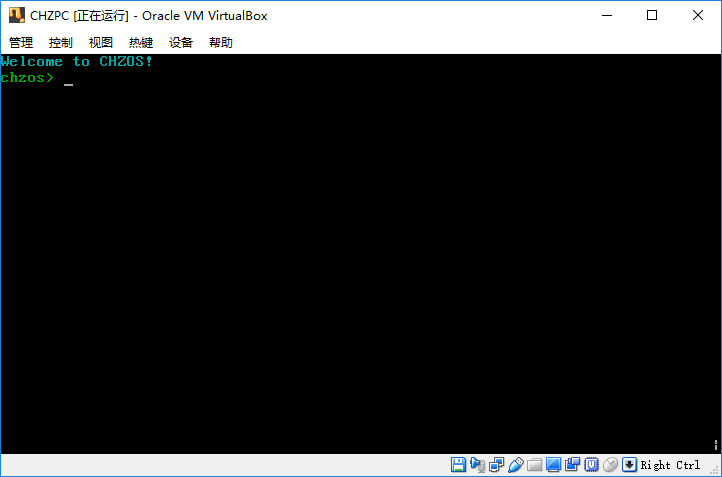
\includegraphics[width=0.5\linewidth]{fig/wheel_1.PNG}&
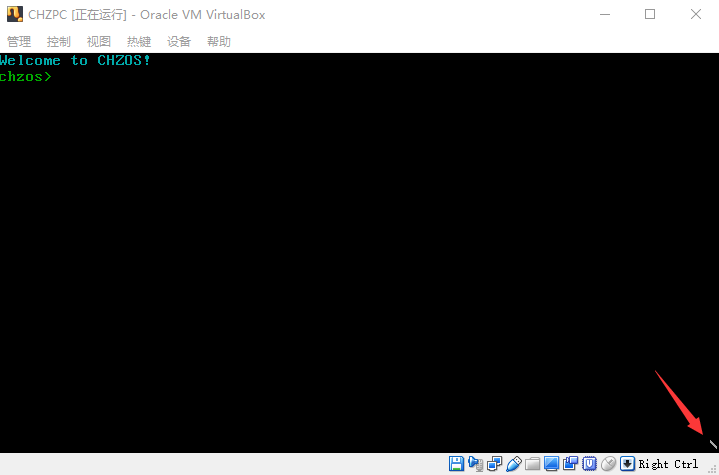
\includegraphics[width=0.5\linewidth]{fig/wheel_2.PNG}\\
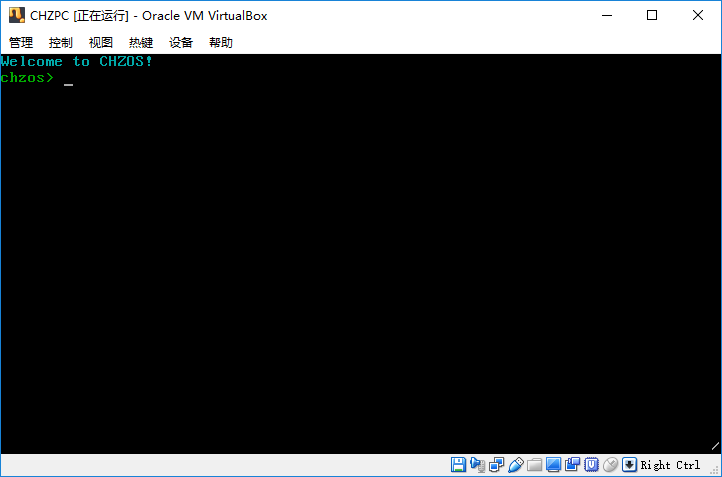
\includegraphics[width=0.5\linewidth]{fig/wheel_3.PNG}&
\end{tabular}
\caption{无敌风火轮}
\label{fig:wheel}
\end{figure}

所有用户程序执行过程中,碰到按键会在屏幕中间红色高亮显示``OUCH!OUCH!'',如图\ref{fig:ouch}所示。
\begin{figure}[H]
\centering
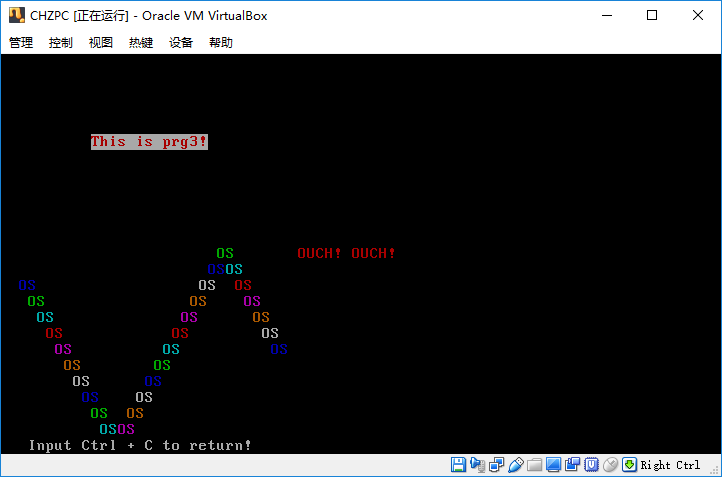
\includegraphics[width=0.8\linewidth]{fig/ouch.PNG}
\caption{键盘中断显示}
\label{fig:ouch}
\end{figure}

连续依次调用\verb'int 33h'、\verb'int 34'、\verb'int 35'和\verb'int 36'中断,这里为了显示方便,没有添加清屏指令,结果如图\ref{fig:int_4}所示。
注意这几条指令都是顺序执行的,即中断调用可\textbf{正常返回父程序},并进入下一行执行,所以才有办法保持原程序产生的结果不发生改变。
\begin{figure}[H]
\centering
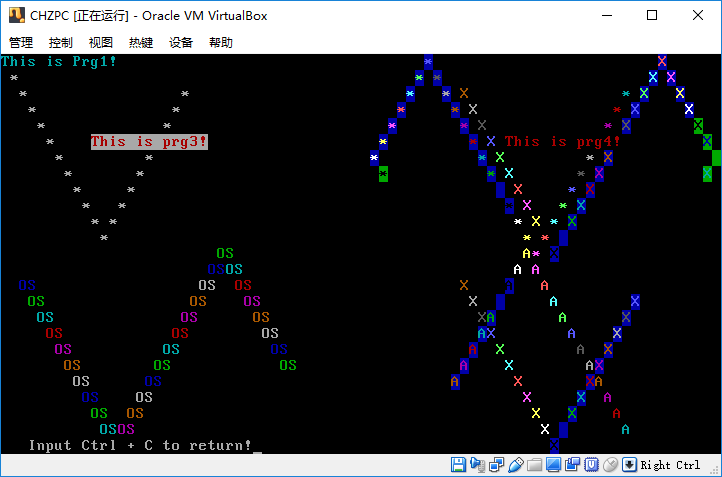
\includegraphics[width=0.8\linewidth]{fig/int_4.PNG}
\caption{连续中断调用}
\label{fig:int_4}
\end{figure}

自动滚屏如图\ref{fig:sroll_down}所示。
可以见到最上面上一次\verb'help'的输出结果被截断了。
\begin{figure}[H]
\centering
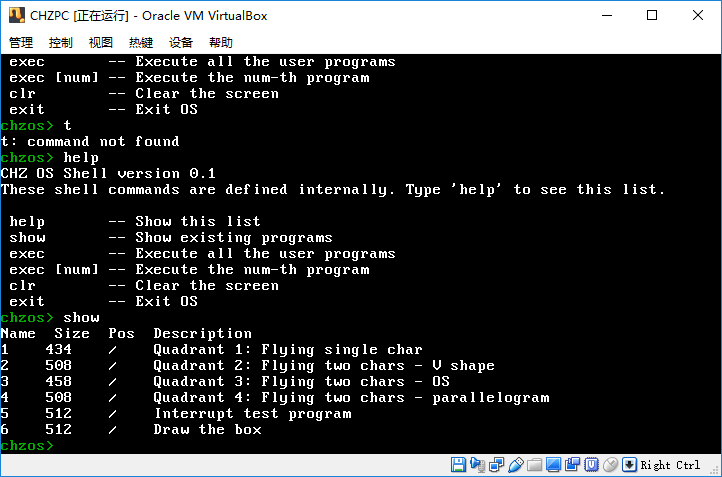
\includegraphics[width=0.8\linewidth]{fig/sroll_down.PNG}
\caption{自动滚屏}
\label{fig:sroll_down}
\end{figure}

由于无敌风火轮已经占用了时钟中断,故自动画框变为用户程序,效果如图\ref{fig:box}所示。
\begin{figure}[H]
\centering
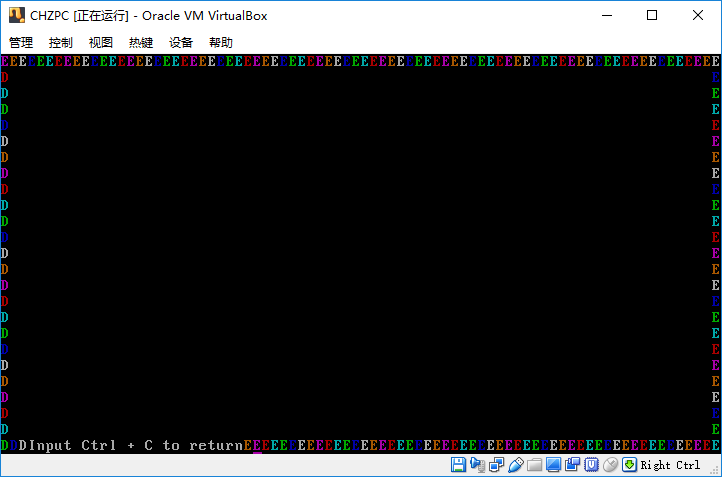
\includegraphics[width=0.8\linewidth]{fig/box.PNG}
\caption{自动画框}
\label{fig:box}
\end{figure}

\section{实验总结}
% 每人必需写一段,文字不少于500字,可以写心得体会、问题讨论与思考、新的设想、感言总结或提出建议等等。不得抄袭,否则按作弊处理。

由于实验二我已经自行实现了中断,因此宏汇编代码可以复用,本次实验就比较简单。

但还是遇到了很多问题,原来我写用户程序时,都没有将其当成一个函数,即最后都是陷入死循环\verb'jmp $',而不是返回原处。
如果用户程序嵌套调用,或者直接在用户程序中调用中断,那很可能回不到原来的断点。
这对于正常的用户程序运行显然是不行的。
因而我认真学习了C编译出来的汇编代码,发现它每一个编译出来的函数体都一定会有\verb'ret'函数,主函数\verb'main'也是,这导致外部程序可以很方便地\verb'call'。
因此,我认为我自己写的用户程序也应该是这样,于是便在我的每一个用户程序的主函数中添加\verb'ret'指令。

但这里很重要一点在于不能破坏堆栈,一旦在用户程序执行中堆栈被破坏,\verb'ret'指令就不能正确找到返回地址,因而跳转到非法位置。
这一点我也单步调试了很长时间,最终发现不管哪一个段寄存器被修改了(因为在显存显示时需要设置段地址,故段寄存器会改变),原来的堆栈就会被修改。
因此,在每次显示字符之前需要将段寄存器\verb'es'、\verb'gs'进栈,显示完后再将段寄存器出栈,这样就可以保证堆栈不会被破坏,最终\verb'ret'可以正常返回父用户程序。

另一个麻烦的点在于,时钟中断总是会和其他中断冲突(主要是读入字符的\verb'int 16'中断)。
查了很多资料,设置好中断处理规则(关中断、中断处理、开中断),倒腾了很久,最终才终于实现两者都能工作。

总的来说,本次实验还是比较轻松愉悦的。

\section{参考资料}
\begin{enumerate}
	\item 李忠,王晓波,余洁,《x86汇编语言-从实模式到保护模式》,电子工业出版社,2013
	\item 周杰英,张萍,郭雪梅,黄方军,《微机原理、汇编语言与接口技术》,人民邮电出版社,2011
	\item Little OS Book, \url{https://littleosbook.github.io/book.pdf}
	\item Interrupts, \url{https://wiki.osdev.org/Interrupts}
	\item 8259 PIC, \url{https://wiki.osdev.org/PIC#Programming_the_PIC_chips}
	\item 函数调用规则,\url{https://www.cs.princeton.edu/courses/archive/spr11/cos217/lectures/15AssemblyFunctions.pdf}
\end{enumerate}

\appendix
\appendixconfig
\section{程序清单}
\label{sec:code}
由于程序太多,请直接见压缩文件。

\section{附件文件说明}
\begin{center}
\begin{tabular}{|c|l|l|}\hline
序号 & 文件 & 描述 \\\hline
1 & \verb'bootloader.asm' & 主引导程序\\\hline
2 & \verb'os.asm' & 内核汇编部分\\\hline
3 & \verb'kernel.c' & 内核C部分\\\hline
4 & \verb'Makefile' & 编译指令文件\\\hline
5 & \verb'link.ld' & 链接文件\\\hline
6 & \verb'bochsrc.bxrc' & bochs调试文件\\\hline
7 & \verb'mydisk.img' & 核心虚拟软盘\\\hline
8$\thicksim$13 & \verb'prgX.asm' & 用户程序\\\hline
14$\thicksim$18 & \verb'/include' & 内核头文件\\\hline
\end{tabular}
\end{center}

\end{document}

% 实验提交内容
% 实验报告:电子版(Word2003的DOC格式或PDF格式)
% 原程序文件及可执行代码程序文件
% 测试输入数据文件和输出数据文件
% 虚拟机软盘映像文件

% 基础实验项目5个和扩展实验7个
% 实验项目,迟交影响成绩评价!
% 工具与环境可由选择,开发新型工具或优化一套开发环境都可加分!
% 一系列基础实验项目必须连续完成,当前项目只能在前一个项目的基础上进行,体现出前后的进化关系,否则要被约谈,证明没有抄袭行为!
% 一个项目可提交多个改进的版本,实现新功能和个性化特征都有利于提高相应项目的成绩。
% 实验项目提交内容用winrar工具整体压缩打包,统一格式命名为:
%    <学号>+<姓名>+<实验项目号>+<版本号>.rar
%    姓名(学号)实验NvX.zip
%    实验报告、项目文件夹、映像文件
%    ftp://172.18.216.232 sysuac 下周六23:59

% 免考
% 条件:实验1~6全部评价AAAAB+B+或相当
% 最终成绩可能范围:75分以上